%
% $Id: ch03_thework.tex
%
%   *******************************************************************
%   * SEE THE MAIN FILE "AllegThesis.tex" FOR MORE INFORMATION.       *
%   *******************************************************************
%
\chapter{Implementation} \label{ch:method}
This chapter provides an overview of the implementation of the Go and Hex classes, the game-playing agents, and the games framework.  Furthermore, we outline our experiments and the methods of running these experiments; the results of the experiments will be discussed in the next chapter.  In each section, we provide both high-level descriptions of the relevant code structure as well as in-depth, low-level discussion of any important algorithms.  The chapter is organized such that the entire code structure is explained from the inside out.  That is, we first describe the games, then the agents which play the games, and finally the framework which orchestrates the playing of the games.  This is because an understanding of each of these parts of the implementation is beneficial to understanding the following parts.

Before the discussion of the more involved classes, we need to first explain the \texttt{Board.java} class, a very simple object which is used in almost every other class.  The \texttt{Board} object provides a representation of a game-independent game board --- there is no game-specific functionality in a \texttt{Board} object.  A \texttt{Board} consists of a 2-dimensional \texttt{char} array which represents a physical game board, and an \texttt{int} to hold the size of the board.  

The constructor for \texttt{Board.java} takes an \texttt{int} as input which sets the size of the board.  The constructor then initializes the 2-dimensional \texttt{char} array with the number of rows and columns both equal to the size of the board.  Every index of the array is set to the dash character (`--') to represent an unoccupied space of the board.  When a player places a piece on the board, an `X' or `O' is placed at the appropriate index of the array depending on whether the move is made by the first or second player, respectively.  \texttt{Board.java} consists of instance methods to get/set each instance variable, print the board to the console, and place either an `X' or an `O' at a given index.

\section{Games}
Go and Hex each have a corresponding java class: \texttt{GoGame.java} and \texttt{HexGame.java}, respectively.  Both of these classes are extentions of the abstract class \texttt{Game.java}.  The purpose of these classes is to provide the game-playing agents and games framework with a set of helper methods. \texttt{GoGame.java} and \texttt{HexGame.java} provide game-specific functionality which aids the agents in their move-making process, and helps the manager track the score of the game and change the board between moves, if necessary.

\texttt{Game.java} consists of the following abstract methods which are overridden in \texttt{GoGame} and \texttt{HexGame}:
\begin{itemize}
\item Name: \texttt{getPossibleMoves}\\
Arguments: \texttt{Board board, boolean firstPlayer}\\
Returns: \texttt{ArrayList<Board>}\\
Given a \texttt{Board} and a boolean indicating which player's turn it is on, this method returns an ArrayList of possible boards for the player to move to

\item Name: \texttt{gameFinished}\\
Arguments: \texttt{Board board, int moveNumber}\\
Returns: \texttt{boolean}\\
Returns true if the game should end for the given \texttt{Board} and move number

\item Name: \texttt{calculateScore}\\
Returns the score of the given \texttt{Board}\\
Arguments: \texttt{Board board}\\
Returns: \texttt{int}\\
Calculates and returns the score of the given \texttt{Board}

\item Name: \texttt{randomPlayout}\\
Arguments: \texttt{Board board, boolean firstPlayer, int moveNumber}\\
Returns: \texttt{int}\\
Performs a random playout from the given \texttt{Board} and returns the score

\item Name: \texttt{randomBoardAfterXMoves}\\
Arguments: \texttt{int boardsize, int moves}\\
Returns: \texttt{Board}\\
Generates a \texttt{Board} of the given size after the given number of random moves have been made on an empty board

\item Name: \texttt{resolveBoard}\\
Arguments: \texttt{Board board, int boardSize}\\
Returns: \texttt{Board}\\
Alters the board after a move is made if needed (e.g. if a move in a game of Go results in a piece being surrounded, this will remove the surrounded piece from the board) and returns the altered \texttt{Board}
\end{itemize}

For both \texttt{GoGame} and \texttt{HexGame}, the \texttt{getPossibleMoves} method is implemented by simply iterating through the board, and attempting to place a piece on each spot as seen in Figure \ref{fig:getPossibleMoves}.  The \texttt{gameFinished} method is implemented differently for \texttt{GoGame} and \texttt{HexGame}.  The method will return true in \texttt{GoGame} if the moveNumber argument exceeds a set number (i.e. the max number of moves has been played; for our experiments we set this to 250), or if both players have no legal moves remaining on the board.  \texttt{HexGame} returns true if the board is completely filled, or the win condition is met for one of the players (this is checked using a simple depth-first search from each edge of the board to the opposite side).

\begin{algorithm}[htbp]
 %\SetLine % For v3.9
 \SetAlgoLined % For previous releases [?]
 \SetKwInOut{Input}{input}\SetKwInOut{Output}{output}
 
 \Input{Board b, boolean firstPlayer}
 \Output{ArrayList$<$Board$>$}
 Initialize empty ArrayList$<$Board$>$\;
 \For{each space on b}{
  \eIf{char at current space on b == `--'}{
   create copy of b\;
   place current player's piece at current space on copy of b\;
   copy of b = resolveBoard(copy of b)\;
   Add copy of b to List\;
   }{
   // do nothing\\
  }
 }
 return ArrayList of boards\;
 \caption{getPossibleMoves pseudocode for both \texttt{GoGame} and \texttt{HexGame}}
\label{fig:getPossibleMoves}
\end{algorithm}

For \texttt{HexGame}, the \texttt{calculateScore} method simply returns 1 if the first player wins, -1 if the second player wins, and 0 if the game has no winner.  For \texttt{GoGame}, score is calculated using the stone-scoring scheme described in Chapter 1, and has a trivial implementation.  The \texttt{randomPlayout} and \texttt{randomBoardAfterXMoves} methods also have a trivial implementation which utilizes \texttt{getPossibleMoves} and Java's \texttt{util.Random} for both games, and \texttt{resolveBoard} simply returns the \texttt{Board} argument in \texttt{HexGame} (there is never a need for board resolution in Hex as pieces are never removed).

However, the \texttt{resolveBoard} method for \texttt{GoGame}, which is used to remove surrounded regions of stones from the board, is more involved.  The algorithm we created for this is based on the flood-fill algorithm \cite{torbert} which is commonly used for the ``paint bucket'' tool of image editing software to fill similarly colored regions with a new color.  A recursive approach is commonly used for this type of algorithm \cite{torbert}, but for the problem of resolving Go boards, we decided a Queue-based approach would be a better method.  A board is resolved by running the algorithm in Figure \ref{fig:resolve} for each occupied space of the board.  Note that in Figure \ref{fig:resolve}, a ``pair'' refers to an (x,y) coordinate pair corresponding to an index of the board.

Essentially, we move outwards along the row of the starting Pair in both directions until the char at both points on the board is no longer equal to the char at the starting point.  We replace every point we visit with a placeholder (the char `A'), and then repeat these actions for the Pairs above and below each visited Pair if their char is equal to the starting Pair.  We do this until we have no more Pairs on which to perform these actions.  If any Pair we visit contains an `--', we know the region is not surrounded and we can return the original Board.  If we never visit a Pair containing an `--' before exhausting all the connected Pairs, we know the region is surrounded; in this case we remove all the `A's from the board, and return.

\begin{algorithm}[htbp]
 %\SetLine % For v3.9
 \SetAlgoLined % For previous releases [?]
 \SetKwInOut{Input}{input}\SetKwInOut{Output}{output}
 
 \Input{Board b, Pair p}
 \Output{Board}
 char c = char at p\;
 Initialize empty Queue$<$Pair$>$ q\;
 q.enqueue(p)\;
 Create Pairs w and e\;
 \While{(!q.isEmpty())}{
  Pair pair = q.dequeue()\;
  Set w and e equal to pair\;
  Decrement x-value of w until char at w != c\;
  Increment x-value of e until char at e !=c\;
  \For{each Pair n between w and e}{
   \If{char at n == `--'}{
   	return original board (area not surrounded)\;
   }
   Replace char at n with `A' (placeholder)\;
   Enqueue Pair north of n if its char == c\;
   Enqueue Pair south of n if its char ==c\;
  }
 }
 Replace every `A' on the board with `--'\;
 return resolved Board\;
 \caption{Board resolution algorithm for \texttt{GoGame}}
\label{fig:resolve}
\end{algorithm}

\section{Game-playing Agents}
Similar to our games, each of the game-playing agents are the children of an abstract class called \texttt{GameAgent.java} (Figure \ref{fig:agentdiag}).  A \texttt{GameAgent} contains a \texttt{Game} object to help it make moves, a boolean tracking whether the agent is the first or second player, an int to track how many iterations of its search algorithm it has gone through (if applicable), and a Random object.  In total, we have five agents extending \texttt{GameAgent}.  The first is a trivial agent which simply makes random moves, called \texttt{RandomAgent}.  The second is \texttt{MCTSAgent} and uses MCTS with a UCT tree policy to inform its move selection.  The other three use MCTS in conjunction with either a genetic algorithm (\texttt{GAAgent}), an artificial neural network (\texttt{ANNAgent}), or the NEAT algorithm (\texttt{NEATAgent}) to modify the search and move selection process.  Each non-trivial agent contains a \texttt{makeMove} method which spends a given amount of time deciding what move to make on a given \texttt{Board}, using various helper methods within the agent.

\begin{figure}[h]
\centering
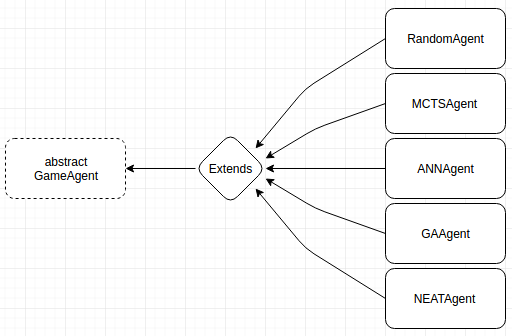
\includegraphics[scale=0.5]{images/gameagent.png}
\caption{Hierarchy of agent implementation}
\label{fig:agentdiag}
\end{figure}

The four non-trivial agents utilize MCTS as the base of their decision-making algorithm, and each have a different Tree policy or Default policy from one another.  Each of the four non-trivial agents follow the four steps of MCTS as outlined in Chapter 1, but each agent may have a slight alteration or addition to the algorithm.  In this section, we describe the way in which we implemented the base MCTS algorithm and \texttt{MCTSAgent}, and then we will look at how each agent modifies this algorithm.  Note that in this next subsection, we will refer solely to the implementation of the \texttt{MCTSAgent} --- however, everything stated directly applies to the other three non-trivial agents as well unless directly stated otherwise when discussing the modified agent.

\subsection{Implementing Monte-Carlo Tree Search}
The main function of MCTS involves incrementally building a tree of possible moves within the game.  For this, we created a \texttt{Node.java} class which behaves slightly differently from how one may expect a generic tree-node to, since it must seperate the children which have been visited in MCTS from those which have not.  Each \texttt{Node} object has the following instance variables:
\begin{itemize}
\item \texttt{double score}\\
Tracks the number of random playouts from this node resulting in a win
\item \texttt{double games}\\
Tracks total number of random playouts performed from this node
\item \texttt{ArrayList$<$Node$>$ unvisitedChildren}\\
Contains all children which have not been visited by MCTS
\item \texttt{ArrayList$<$Node$>$ children}\\
Contains all children which have been visited by MCTS
\item \texttt{ArrayList$<$Node$>$ prunedChildren}\\
Contains nodes pruned (only applicable for ANNAgent)
\item \texttt{Node parent}\\
Points to node's parent
\item \texttt{Board b}\\
The \texttt{Board} associated with the node
\item \texttt{boolean firstPlayer}\\
Tracks who's turn it is on the \texttt{Board} represented by the node
\end{itemize}

\texttt{Node.java} has two constructors, one for the root node of the tree (which is only called on the first iteration of MCTS each turn), and one to create all other nodes.  The root constructor takes a \texttt{Board b} and \texttt{boolean firstPlayer} as arguments and sets the respective instance variables to these values; \texttt{score} is set to 0.0, \texttt{games} is set to 1.0, the children ArrayList is initialized, and its parent is set to \texttt{null}.  The other constructor takes a \texttt{Board b} and \texttt{Node parent} as arguments, and sets the respective instance variables to these.  The only other difference from the root constructor is \texttt{firstPlayer} is set to the opposite of its parent's value.  Each \texttt{Node} has instance methods to find and set its unvisited children, recursively backpropogate scores from random playouts up the tree to the root node, find the UCT value of a node (given an exploration bias parameter as described in Equation \ref{eq:UCT}), and prune nodes from the tree (i.e. remove them from children and/or unvisitedChildren).

Utilizing the \texttt{Node} object, the \texttt{MCTSAgent} is able to build a game tree using MCTS as described in Chapter 1.  In addition to all the instance variables defined in \texttt{GameAgent}, the \texttt{MCTSAgent} also has a \texttt{double explorationConstant} for use in the MCTS algorithm --- for our experiments, this constant was set to $\sqrt{2}$ which provides a rather equal balance between exploration and exploitation \cite{browne2012survey}.  Its \texttt{makeMove} method takes a \texttt{Board b}, \texttt{int timeAllowed}, and  \texttt{int moveNumber} as arguments, which are the current Board, amount of time it is allowed to take to decide on a move, and how many moves have been made in the current game (which is used for random playouts), respectively.

Within the \texttt{makeMove} method is a while-loop which repeatedly calls the agent's \texttt{select} method over its given time allowance.  This method runs through a single iteration of MCTS using various other helper methods --- it selects the node in the tree with the highest UCT value, visits a random one of the node's unvisited children, finds the score of a random playout, and backpropogates it the score up the tree.  Note that with our chosen scoring scheme for Go, the scores of the random playouts can theoretically fall anywhere in the interval $[-s, s]$ where $s$ is the number of cells on the board (e.g. a 9x9 board can have scores anywhere from -81 to 81); however, UCT requires estimated node scores to be in the interval $[0,1]$ \cite{browne2012survey}.  Furthermore, for player two, lower scores are better.  Thus after finding the score of a random playout from a node, we must alter the score before backpropogating it up the tree.

This was a simple process.  First, if the player performing the random playout was the second player, we multiplied the estimated score of the playout by -1.  Then the score was normalized using Equation \ref{eq:norm}, where $s$ is the score of the game on a $b\times b$ Go board.  $s'$ is then the score which is backpropogated up the tree.

\begin{equation}\label{eq:norm}
s' = \frac{s + b^2}{2b^2}
\end{equation}

After the agent spent its alotted amount of time searching the tree, it makes its final move selection.  For final move selection, the agent simply chooses the child of the root with the highest average playout score (i.e. the child with the highest score divided by total games).

\subsection{ANNAgent}
The \texttt{ANNAgent} behaves exactly the same as the \texttt{MCTSAgent} with one caveat: prior to building the game tree with MCTS, it prunes a number of the root's immediate children from the tree.  This is done by training a simple feed-forward network to rank a node's children in order of how likely they are to be repeatedly visited by MCTS --- those with the lowest scores are not included in the search process.  An exponentially decaying pruning scheme is used as outlined in \cite{annpruning}, meaning the number of nodes pruned from the tree exponentially decays as the game progresses.  Using equation \ref{eq:prune} to determine the number of nodes to prune, the agent removes 50 percent of children at move 0, 10 percent of children by move 70, 4 percent by move 125, etc.

\begin{equation}\label{eq:prune}
(\textrm{\% pruned}) = 50 - 48.6*(1 - e^{(-0.0244*x)})
\end{equation}

Seperate neural networks were created and trained for each boardsize of both Go and Hex prior to any experimentation.  In total, 8 neural networks were made (9x9, 11x11, and 14x14 Hex; 5x5, 7x7, 9x9, 11x11, and 13x13 Go).  For this, the Encog machine learning library was used \cite{encog}.  The neural networks were designed as follows for each game on each $n\times n$ board:
\begin{itemize}
\item Input layer consisting of $n\times n$ neurons --- each neuron corresponds to exactly one spot on a board;
\item A single hidden layer consisting of the number of neurons in the input layer divided by 3;
\item Output layer consisting of a single neuron, representing the estimated value of the input board.
\end{itemize}

Only sigmoid activation functions were used in the neural networks, as this was found to provide the best performance for evaluating Go boards by Burger \etal \cite{annpruning}.  We chose a single hidden layer as Heaton, the creator of Encog, suggests that more than a single layer is completely unnecessary for training simple feed-forward networks \cite{encog}.  Finally, we settled on the size of the hidden layer empirically, by briefly testing several hidden layer sizes between that of the input size and output size.

After designing the networks, each network was trained on a seperate set of 2500 randomly generated boards of the network's respective game type and board size.  Each set contained an equal number of boards representing random games after 5 moves, 10 moves, 15 moves, etc. up to 105 moves.  In order to estimate the value of each of these boards, an \texttt{MCTSAgent} performed 10,000 iterations of MCTS for each board; the UCT value of each board after 10,000 iterations was used as the ideal output value for the input board.  

We chose to train each network on this dataset until the network's error was below 0.0001 --- this seems like an incredibly low amount of error, but such a low error was actually necessary to guarantee any level of accuracy from our networks.  Because of our randomly generated inputs for each dataset and the large number of MCTS iterations, most of the ideal values were found to be between 0.45 and 0.55.  Such a small range in most of the training data meant that a calculated level of error would in actuality be magnitudes higher.  For example, if the network were to classify every single input as having a value of 0.5, the error would likely only read to be around 0.05 since most of the ideal values are between 0.45 and 0.55 --- such a network is clearly far from being accurate, despite having a seemingly low error over the training set.

After being trained, the networks were each serialized using Java's serialization library.  The \texttt{ANNAgent} has a \texttt{BasicNetwork} instance variable (imported from the Encog library) which is initialized upon creation of the agent.  Before gameplay, the agent chooses the appropriate network to deserialize based on the gametype and size of the game board.  On each turn, the agent then uses this network to evaluate moves and remove a percentage of them from the game tree, as described earlier.

The process of evaluating each child of the current board, sorting them by estimated ranking, and removing a set number of them from the tree obviously takes some of the agent's alotted time that could be spent performing more iterations of MCTS.  So, what is expected to be gained by this process?  Essentially, the idea behind the \texttt{ANNAgent} is that, while it performs a lower number of iterations of MCTS, more of the iterations it does perform will be done exploring high quality moves.  If we can identify which children will not be explored heavily before even starting MCTS, the number of iterations lost from time spent evaluating children may be overcome by the fact that any iterations of MCTS that would have been wasted exploring those moves can now be spent on deciding between fewer, better options.


\subsection{GAAgent}
The \texttt{GAAgent} utilizes a genetic algorithm to bias both its tree policy and its final move selection.  The agent's genetic algorithm consists of a population of \texttt{GAWeight} objects, which each hold a weight vector of five doubles $(x_1 \cdots x_5)$ between zero and one to represent the weight given to a hueristic property of the game board.  Tables \ref{table:go} and \ref{table:hex} give the names and descriptions of each of the games' heuristic properties which are used.  Each \texttt{GAWeight} also contains methods to evaluate each heuristic property of a given board.

\begin{table}[h]
\centering
\begin{tabular}{|c|l|}
\hline
\textbf{Property name} & \textbf{Definition}\\
\hline
\hline
netStones & Score of resulting board\\\hline
goodLibs & Number of own liberties on board\\\hline
badLibs & Number of opponent's liberties on board\\\hline
goodAtari & Number of own stones in atari\\\hline
badAtari & Number of opponent's stones in atari \\\hline
\end{tabular}
\caption{Properties used for Go genetic algorithm}
\label{table:go}
\end{table}

\begin{table}[h]
\centering
\begin{tabular}{|c|l|}
\hline
\textbf{Property name} & \textbf{Definition}\\
\hline
\hline
netBridges & Net number of bridges on board\\\hline
goodConnected & Size of largest connected region of own stones\\\hline
badConnected & Size of largest connected region of opponent's stones\\\hline
goodDeepest & The smallest number of agent's moves needed to win\\\hline
badDeepest & The smallest number of opponent's moves needed to win\\\hline
\end{tabular}
\caption{Properties used for Hex genetic algorithm}
\label{table:hex}
\end{table}

For example, consider Figures \ref{fig:goheur} and \ref{fig:hexheur}.  These are representations of small boards from Go and Hex, after several moves have been made --- the boards were generated using GoGui \cite{fuego} and HexGui \cite{benzene}, respectively.  On the Go board, the blue dots represent white stones' liberties while the red dots represent black stones' liberties; stones marked with green dots represent stones in atari.  Meanwhile on the Hex board, the blue shaded region represents the largest region of black stones, the red shaded region represents the largest region of white stones, green lines represent any bridges, and the empty spaces marked with `X' represent the spaces where either player would need to play to end the game.

\begin{figure}[h]
\centering
\begin{minipage}{.5\textwidth}
  \centering
  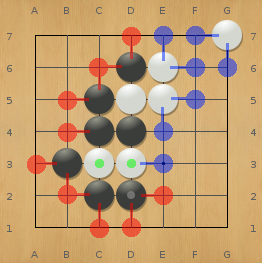
\includegraphics[scale=0.65]{images/goheuredited.png}
  \captionof{figure}{Go heuristic properties}
  \label{fig:goheur}
\end{minipage}%
\begin{minipage}{.5\textwidth}
  \centering
  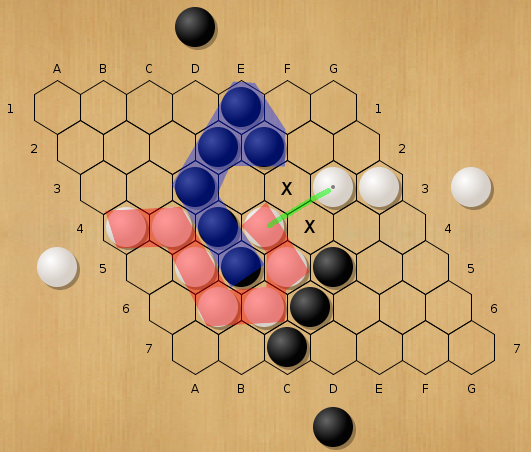
\includegraphics[scale=0.375]{images/hexheuredited.png}
  \captionof{figure}{Hex heuristic properties}
  \label{fig:hexheur}
\end{minipage}
\end{figure}

So, suppose a \texttt{GAAgent} is playing as black in both of these games and one of its \texttt{GAWeights} is evaluating the boards.  For Go, the \texttt{GAWeight} would find a netStones value of -1 (6 white stones and 7 black stones), a goodLibs value of 9, a badLibs value of 7, a goodAtari value of 0, and a badAtari value of 2.  If $(x_1, \cdots, x_5)$ are the respective weights for each property, the \texttt{GAWeight} would find the overall value $v_1$ of the Go board to be 
\[v_1 = -1x_1 + 9x_2 + 7x_3 + 0x_4 + 2x_5.\]
For the Hex board, the \texttt{GAWeight} would find a netBridges value of 1 (1 white bridge and 0 black bridges), a goodConnected value of 6, a badConnected value of 7, a goodDeepest value of 2 (both spots marked x needed to win for black), and a badDeepest value of 1 (only one spot marked x needed to win for white).  So, the \texttt{GAWeight} would find the overall value $v_2$ of the Hex board to be
\[v_2 = 1x_1 + 6x_2 + 7x_3 + 2x_4 + 1x_5.\]

When a \texttt{GAAgent} is created before the start of a game, it is given a small population of 10 \texttt{GAWeights} with randomized weight vectors $(x_1 \cdots x_5)$.  While, traditionally, a genetic algorithm requires each member to fully complete its task (e.g. play a full game of Go) in order to evaluate a member's fitness, the nature of MCTS allows us to to evolve the weight vectors many times during a single game \cite{lucas2014fast} --- rather than use a full, real playout of a game the fitness of a \texttt{GAWeight}, we can use the simulated playouts of a game during each iteration of MCTS.

We evaluate, select, crossover, and mutate the population of \texttt{GAWeights} after every 100 iterations of MCTS; each of the ten \texttt{GAWeights} is used ten times to bias the \texttt{GAAgent} before evaluation.  So, when the \texttt{GAAgent} is asked to make a move, it selects a node of the tree to expand taking into account both the UCT scores and estimated board values of each node.  A random playout is performed from the chosen node as usual, and, for the purpose of fitness evaluation, the score of the playout is stored in whichever \texttt{GAWeight} was used.  After every 100 iterations of MCTS, each \texttt{GAWeight} will have been used 10 times and we can perform the evolutionary algorithm on the population.

Evaluating the fitness of the population is simple; we look at the saved playout scores of each \texttt{GAWeight}, and a higher average score equates to a higher fitness.  The two \texttt{GAweights} with the lowest fitness are removed from the population and are replaced by two children of the highest performing \texttt{GAWeights}.  These children are made by simply averaging the weight vectors of the parents --- prior to mutation, the two children are exactly the same.  Mutation of each child is done independently on each of its weights --- if a weight is chosen to be mutated, it is averaged with a random double between 0 and 1.

For the first child, each weight has a 20\% chance of being mutated, while each weight of the second child has a 60\% chance of being mutated.  So, on average, one of the first child's weights will be mutated while three of the second child's weights will be mutated.  We chose these high mutation rates because of the small population size and the small number of random playouts performed relative to the branching factor of each game.  A high mutation rate keeps the population diverse and allows the agent to more easily discover heuristic strategies far different from those in the starting population.

After the \texttt{GAAgent}'s alotted time to decide on a move is up, it biases its final move selection as well.  The agent assigns a score to each possible move in the same way as the \texttt{MCTSAgent}, biases each move with the highest performing \texttt{GAWeight} in its population, and selects the move with the highest final score.  During both the selction phase of MCTS and final move selection, the \texttt{GAAgent} essentially introduces a small amount of heuristic analysis into its decision making in order to differentiate between nodes in the tree with similar UCT scores.  We observed that during MCTS, there are oftentimes several clusters of nodes which have similar UCT scores.  Hypothetically, the \texttt{GAAgent} should be able to choose between similarly scoring moves more accurately; this could be particularly helpful when the agent is only able to run through a small number of iterations of MCTS (e.g. early in a game of Go on one of the larger boards).

\subsection{NEATAgent}
Rather than alter the MCTS tree policy or final move selection like the previous agents, the \texttt{NEATAgent} uses an evoloved neural network to alter the default policy of MCTS as proposed by Gauci and Stanley in \cite{hyperneatgo}.  The logic behind this agent is that, when playing against a non-trivial player, a random playout will likely not result in a very accurate representation of a game playout.  Thus, a default policy which chooses moves more intelligently will allow the MCTS algorithm to better estimate the scores of playouts during the simulation phase.

Gauci and Stanley proposed using NEAT to create a network which acts as an action selector --- given a board, the network provides each empty space with a score based on how valuable placing a piece at that spot would be.  The Encog framework \cite{encog} provides NEAT functionality and was used to implement this system.  Similar to the ANNs created for \cite{ANNAgent}, a different network was created for each boardsize of each game, and each have an input layer size equal to the number of spots on the board (e.g, 81 input neurons for a game on a 9x9 board).  Because these networks are acting as an action selector, the size of the output layer is also equal to the number of spots on the board --- each output neuron represents the value of placing a piece at the spot represented by the input neuron in the same place.  The networks were limited to using only sigmoid activation functions.

To train the networks, we again randomly generated 2500 boards of the appropriate game and board size for each.  For each board, an \texttt{MCTSAgent} performed 5000 iterations of MCTS using the board as the root of the tree.  This allowed us to estimate the value of each legal move by looking at the score of each of the board's children.  The ideal value for the output of the board was set to the corresponding move's score; any output neurons which represented spaces which were not valid moves had the ideal value set to 0.  

After the training dataset was created, each network was trained until its error was below 0.1.  The networks were then serialized using Java's serialization library, and the \texttt{NEATAgent} contains a \texttt{NEATNetwork} instance variable, similar to the \texttt{ANNAgent}.  Upon creation, the \texttt{NEATAgent} can pick the appropriate network to use, and assign the network to this instance variable.  During MCTS, the \texttt{NEATAgent} has a standard selection and expansion phase.  For the simulation phase, though, the agent uses a built-in playout method called \texttt{biasedPlayout} rather than the random playout functionality provided in the games classes.

The \texttt{biasedPlayout} method takes a \texttt{Node} as input (the node which is expanded to during MCTS), and returns a score of a playout from this \texttt{Node}.  During each move of the simulated playout, the agent evaluates the current board with its network and places a piece at the spot corresponding to the output neuron with the highest value.  The agent's MCTS process is otherwise the same as the standard \texttt{MCTSAgent}, calculating the score at the end of the playout and backpropogating it up the tree.  The agent's final move selection is also the same, selecting the move with the highest ratio of average-playout-score to total-games-simulated.

\section{Games Framework}
\texttt{GameController.java} is the ``runner'' class of our framework and orchestrates the actual playing of games --- it is used to create game and agent objects, run the games, and record data.  In order to run this program, note that you must include the \texttt{encog-core-3.3.0} and \texttt{jcommander-1.48} JARs included in the \texttt{/lib} directory of the project.  The class contains a \texttt{Game} object, a \texttt{Board} object which acts as the master game board, two \texttt{GameAgent} objects, and several \texttt{FileWriters} to record data.  We parse command-line inputs using the JCommander library \cite{jcommander} to determine gametype, board size, which agents are playing, etc. (Table \ref{table:jco}).  Our framework also supports human play by printing the game board to the terminal between moves, and allowing human players to make moves by typing the row and column of the space on which they wish to place their piece.

\begin{table}[h]
\centering
\begin{tabular}{|l|c|l|}
\hline
\textbf{Parameter} & \textbf{Default} & \textbf{Description}\\
\hline
\hline
String --agent1 & ``human" & Player one's agent type \\\hline
String --agent2 & ``human" & Player two's agent type \\\hline
int --size & 9 &  Size of the game board\\\hline
String --game & ``go" & The game being played \\\hline
int --time & 3000 & How many milliseconds can be spent making a move \\\hline
boolean --record & false & Record game data \\\hline
boolean --help & false & Display JCommander usage \\\hline 
\end{tabular}
\caption{JCommander parameters for \texttt{GameController.java}}
\label{table:jco}
\end{table}

Following the creation of all of the necessary objects, \texttt{GameController} simply enters a \texttt{while-loop} which executes until the game is complete; the game over condition for whichever game is being played is checked following every move.  While the game over condition is not met, each of the two players are simply asked to make a move.  If the player is human, the game halts until a valid move is typed into the terminal; otherwise, the agent's \texttt{makeMove} method is called for the current \texttt{Board}, movenumber, and time allowance.  After each move, if \texttt{--record} has been set to true, the current game score and number of iterations of MCTS the agent was able to complete (if applicable) is written to a .csv file.  Figure \ref{fig:finalframework} illustrates the entire structure of the framework during gameplay between two agents.

\begin{figure}[h]
\centering
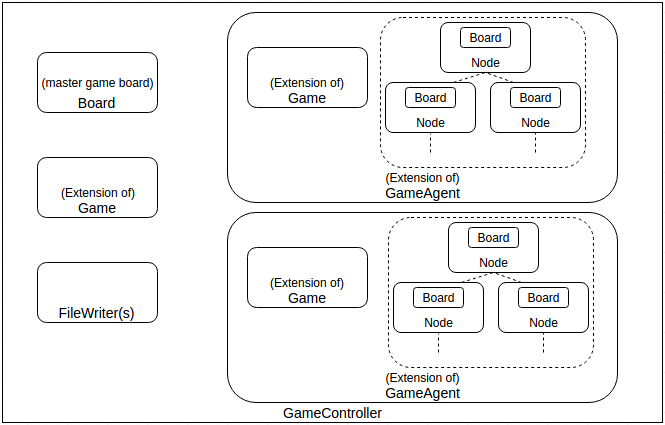
\includegraphics[scale=0.58]{images/finalframework.png}
\caption{Structure of the game-playing framework}
\label{fig:finalframework}
\end{figure}

The entire framework was written with expandability in mind.  The extensive use of object-oriented programming paradigms allows for new games and agents to be integrated into the framework with ease.  Adding support for a new game or agent would require no changes to the existing Java classes, other than adding a few lines to instantiate the new object in \texttt{GameController.java}.

\section{Experiments}
Our experiments consisted of having every agent play one another multiple times on different sized boards of each game under different time allowances.  Each pair of agents played games on 5x5, 7x7, 9x9, 11x11, and 13x13 Go as well as 9x9, 11x11, and 14x14 Hex.  For each of these gametypes, 20 games were played with time allowances of 500ms, 1000ms, 2000ms, 4000ms, and 8000ms.  The goal of running so many variations of the games is to uncover performance trends of each agent relative to one another as the board size and time allowance changes.  The different board sizes provide different branching factors (e.g. 13x13 Go has a much higher branching factor than 7x7 Go), while the different time allowances allow for each agent to run through more iterations of MCTS on each turn.

Because of the large number of experiments, we chose to distribute them over multiple machines in Alden Hall and run them concurrently.  We achieved this by manually \texttt{ssh}ing into a different machine for each pair of agents, and running a simple \texttt{bash} script on each to run 20 games between the two agents for each variation in board size and time allowance.  Each \texttt{bash} script simply sets the classpath to include the necessary JARs, and loops through playing the different games with the \texttt{--record} option set to true.

\section{Threats to Validity}
I think I will have a section on issues with / potential improvements to the project in the final chapter, after the results have been discussed.  That organization makes more sense to me (explain implementation/experiments -$>$ analyze results -$>$ discuss validity of results/improvements to the experiments).  Leaving this here for now so I don't forget about this later if I change my mind.